\subsection*{Part B}
\begin{enumerate}
    \setcounter{enumi}{11}
    \item Windows Firewall can disallow connections from specific applications, or \textbf{outbound rules} can be set to block programs from reaching the internet. Navigate to the \textbf{Outbound Rules} section.
    \item To create a new outbound rule, click the \textbf{New rule} option.
    \item We create a \textbf{Port} rule.
    \begin{figure}[H]
        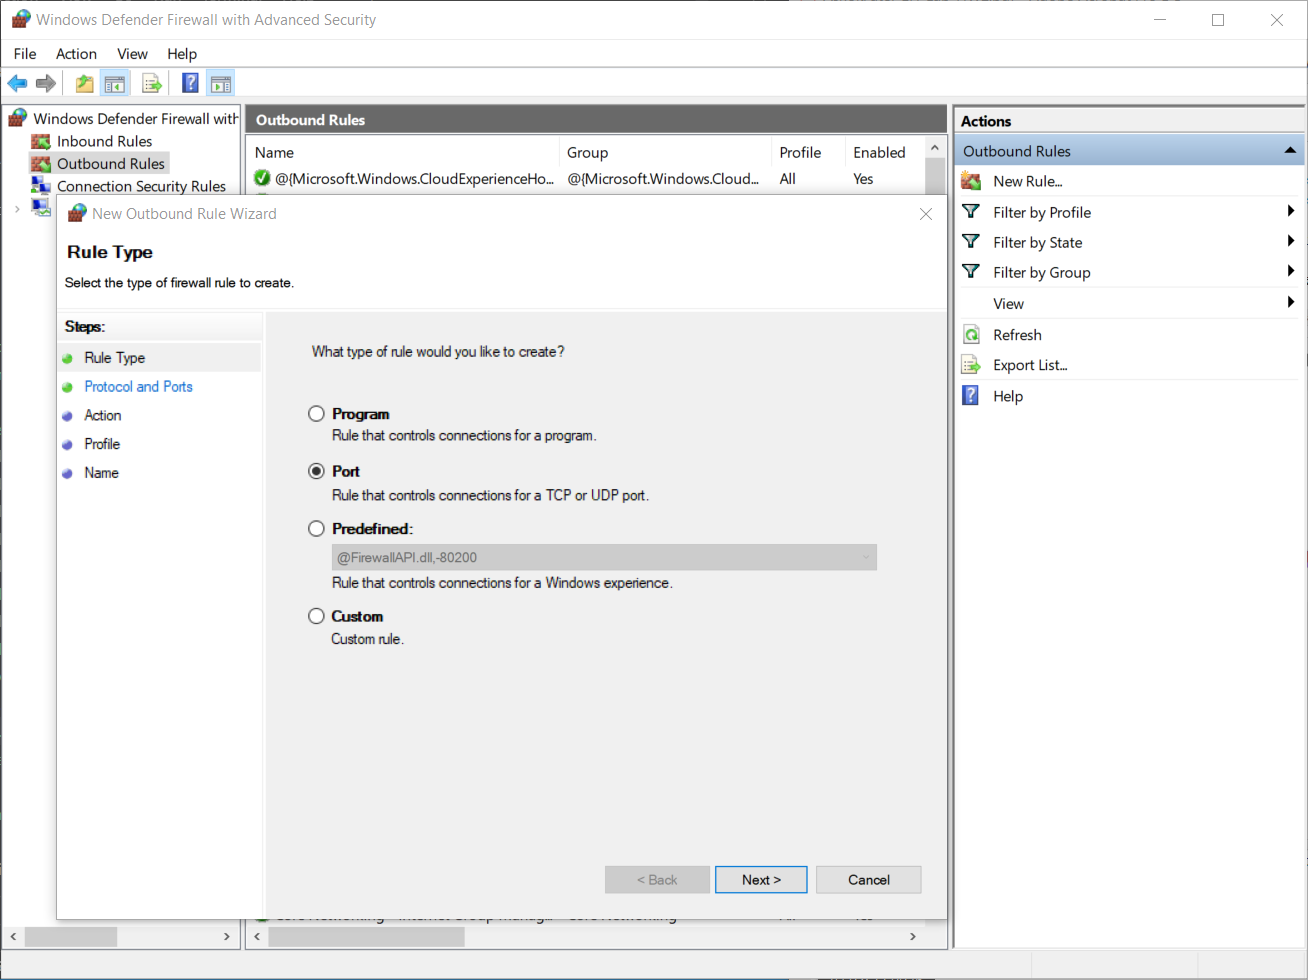
\includegraphics[width=\linewidth]{figures/pic9.png}
    \end{figure}
    \item The rule applies to \textbf{TCP} connections.
    \item Port 80 is the specific port that will be blocked by this rule.
    \begin{figure}[H]
        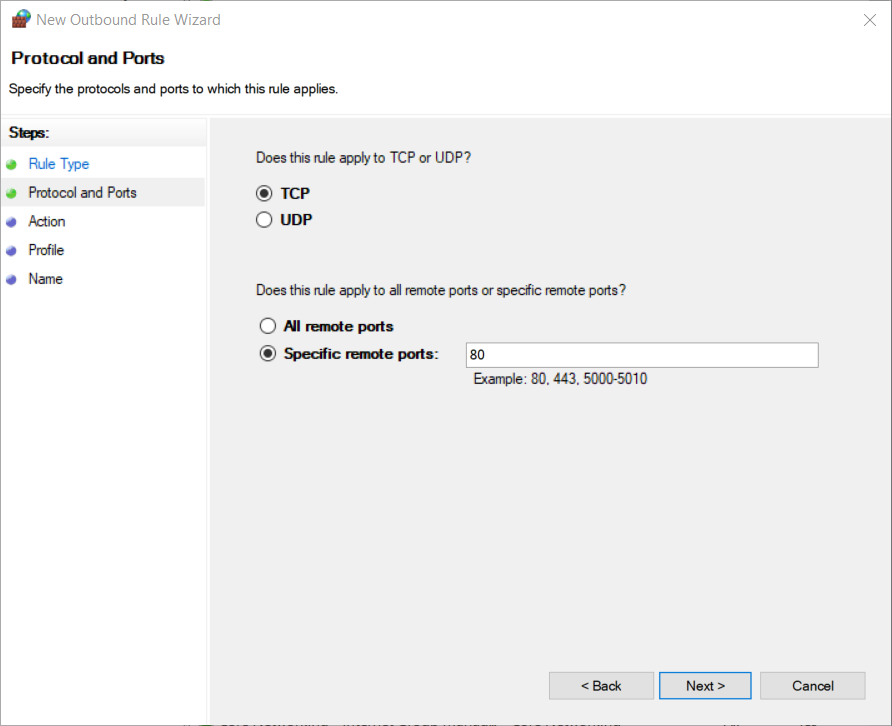
\includegraphics[width=\linewidth]{figures/pic10.png}
    \end{figure}
    \item With the port specified, \textbf{Block the connection} is selected to disable the port.
    \item We apply the rule to all three firewall domains: Public, Private and Domain.
    \item We name the rule \textbf{Block Port 80} to finalize the creation.
    \item Attempting to connect to a website using an \textbf{HTTPS} connection is still allowed because the connection does not use port 80.
    \begin{figure}[H]
        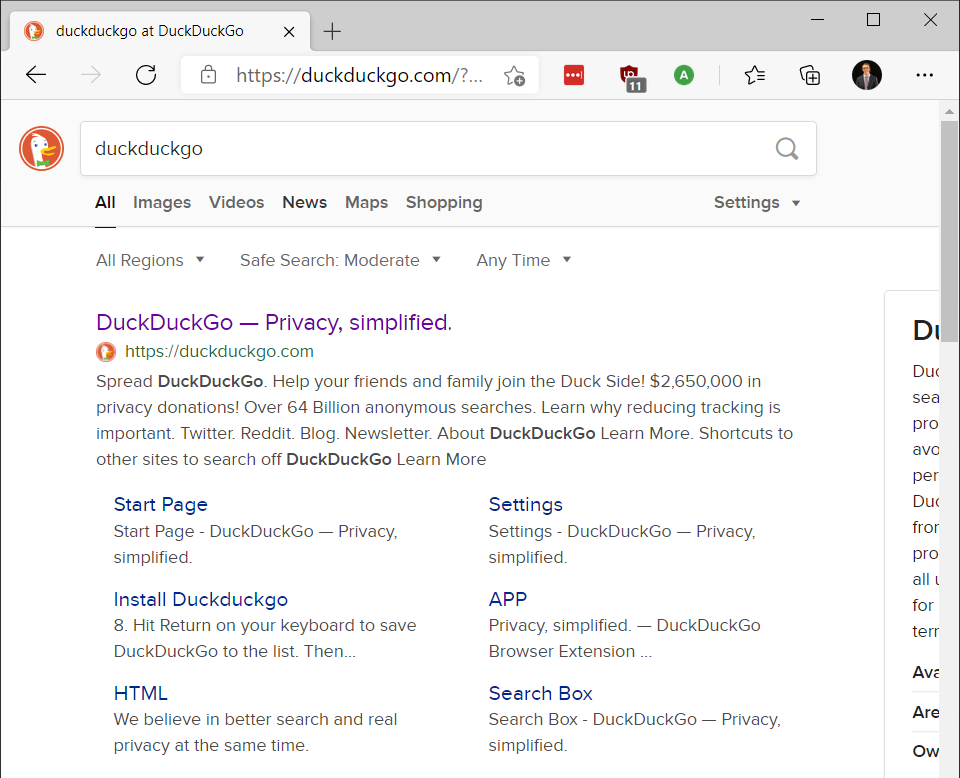
\includegraphics[width=\linewidth]{figures/pic11.png}
    \end{figure}
    \item While connecting using \textbf{HTTP} the access is blocked because port 80 is not enabled, thus not allowing traffic to the website.
    \begin{figure}[H]
        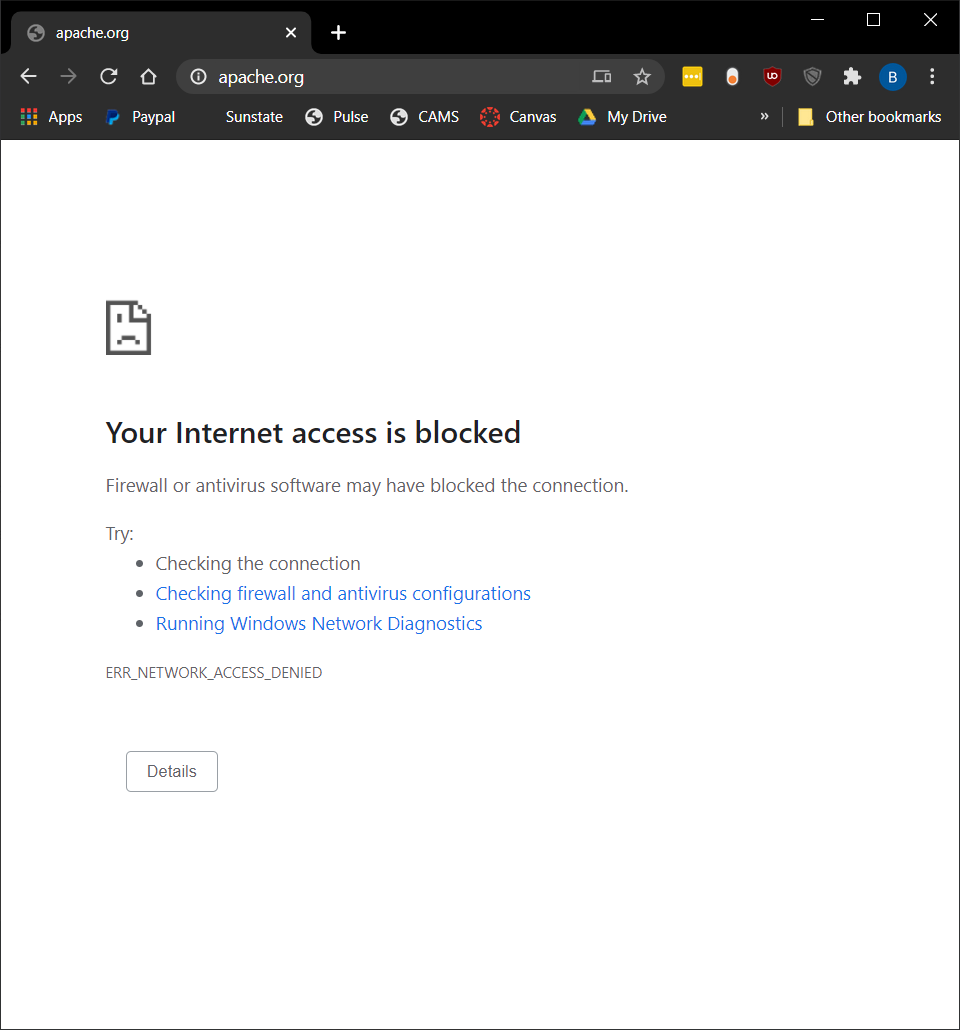
\includegraphics[width=\linewidth]{figures/pic12.png}
    \end{figure}
\end{enumerate}